\section{Total Least Squares (TLS)}
\subsection{Theory}
Total Least Squares solves a nonlinear, overconstrained system of equations by minimizing the squared residuals of each observation.  A Taylor Series expansion is utilized to linearize the equation and iteratively calculate the gradient of the function to determine a local minima.  A Weight Matrix, with a column/row for each observation rather than observation equation, is used to allow for error in all dimensions.  Traditionally, this will be a predicted variance for each observation.

*Note that if the scale of the variance-covariance in the weight matrix is known to be 1, then the computed reference variance should be inspected to ensure it passes the $\chi^2$ goodness of fit test.  If it passes the test, the Covariance matrix should NOT be multiplied by the reference variance.  See definition of reference variance for the reasoning.

\subsection{Assumptions}
\begin{itemize}
	\item No Outliers/Blunders. Nonlinear Least Squares is not robust to outliers (consider RANSAC/Robust Weighting if outliers)
	\item System is over-constrained (eg. Number of Observation Equations > Number of Unknowns)
	\item Error is in all measurements variable (eg. mx+b = y + v $\rightarrow$ error only in x and y dimension)
	\item $X_0$ must be a reasonable guess, otherwise the solution might settle on an incorrect local minima, rather than the global minimum.  If a linear problem, one method is to solve the unweighted OLS, then use that to initialize $X_0$ in TLS.
\end{itemize}
\subsection{Equations}
\[
\hspace{5cm} AX=L \hspace{1cm} \text{(note: residuals in both X and L)}
\]
\[
BV + J\Delta X = K 
\]
\[
m = \text{number of observations} \hspace{1cm} 
n = \text{number of unknowns} \hspace{1cm}
\]
\[
p = \text{number of observation equations for each observation}
\]
\[
q = \text{number of input variables}
\]
\[
dof = \text{degrees of freedom (\# of redundant observations)} = m-n
\]
\[
i = \text{loop iteration}
\]
\[
\text{Observation Equations =  } F_m(x_1,x_2,...,x_n) = l_m \text{ (note: }AX\text{ is obs eqn, L is }[l_1,l_2...,l_m] \text{ )}
\]
\setcounter{MaxMatrixCols}{20}
\[
b(r) = 
\begin{bmatrix}[1.5]
\ddx{F_1}{v_{1r}} & \ddx{F_1}{v_{2r}} & \dots & \ddx{F_1}{v_{pr}} \\
\ddx{F_2}{v_{1r}} & \ddx{F_2}{v_{2r}} & \dots & \ddx{F_2}{v_{pr}} \\
\vdots & \vdots & \ddots & \vdots \\
\ddx{F_k}{v_{1r}} & \ddx{F_k}{v_{2r}} & \dots & \ddx{F_k}{v_{pr}} \\

\end{bmatrix}
\hspace{0.5cm}
B = 
\begin{bmatrix}
b(1) & 0 & \dots & 0 \\
0 & b(2) & \dots & 0 \\
\vdots & \vdots & \ddots & \vdots \\
0 & 0 & 0 & b(m) \\
\end{bmatrix}
\hspace{0.5cm}
V = 
\begin{bmatrix}
v_{11} \\
v_{21} \\
\vdots \\
v_{p1} \\
v_{12} \\
v_{22} \\
\vdots \\
v_{p2} \\
\vdots \\
v_{1m} \\
v_{2m} \\
\vdots \\
v_{pm}
\end{bmatrix}
\]
\[
J = \begin{bmatrix}[1.5]
\ddx{F_1}{x_1} & \ddx{F_1}{x_2} & \dots & \ddx{F_1}{x_n} \\
\ddx{F_2}{x_1} & \ddx{F_2}{x_2} & \dots & \ddx{F_2}{x_n} \\
\vdots & \vdots & \ddots& \vdots \\
\ddx{F_m}{x_1} & \ddx{F_m}{x_2} & \dots & \ddx{F_m}{x_n} \\
\end{bmatrix}
\hspace{0.5cm}
\Delta X = 
\begin{bmatrix}
\Delta x_1 \\ \Delta x_2 \\ \vdots \\ \Delta x_n
\end{bmatrix}
\hspace{0.5cm}
K = 
\begin{bmatrix}
l_1 - F_1(X_i) \\ l_2 - F_2(X_i)\\ \vdots \\ l_m - F_m(X_i)
\end{bmatrix}
\]
\[
\Sigma = 
\begin{bmatrix}
\sigma_{1}^2 & \sigma_{12} & \dots & \sigma_{(1\times n)} \\ 
\sigma_{21} & \sigma_{2}^2 & \dots & \sigma_{(2\times n)} \\ 
\vdots & \vdots & \ddots& \vdots \\
\sigma_{(n\times 1)} & \sigma_{(n\times 2)}^2 & \dots & \sigma_{n}^2 \\ 
\end{bmatrix}
\hspace{1cm}
\text{Initial Guess } X_0 = 
\begin{bmatrix}
x_1 \\ x_2 \\ \vdots \\ x_n
\end{bmatrix}
\]
\subsubsection{Loop Equations:}
Loop until $\Delta X $ is small, or more robustly, loop until $S_0^2$ increases.  $S_0^2$ will increase slightly when you get down to really really small numbers and the cpu starts rounding.  Caveat: it will also increase if you have a really bad initial guess, and it starts diverging.
\vspace{0.15cm}
\begin{align*}
	\text{Equivalent Weight} &=  W_{eq} = inv(B\Sigma B^T) \\
	\text{Loop Delta Estimate} &= \Delta X = inv(J^TW_{eq}J)J^TW_{eq}K \\
	\text{Loop Estimate} &=  \hat{X}_i = X_{i-1}+\Delta X \\
	\text{Equivalent Residuals} &= V_{eq} = K_i \\
	\text{Reference Variance} &= S_0^2 = \dfrac{V_{eq}^TW_{eq}V_{eq}}{dof}
\end{align*}
\todo{make sure V = K in all nonlinear}
\subsubsection{Final Calculations}
\begin{align*}
	\text{Observation Residuals} &= V = \Sigma B^T W_{eq} V_{eq} \\
	\text{Unknowns} &= \hat{X} = \hat{X}_i \text{   (Final Loop Estimate)}\\
	\text{Cofactor Matrix} &= Q_{xx} = inv(J^TW_{eq}J) \\
	\text{Covariance Matrix of Unkowns} &= \Sigma_{xx} = S_0^2 \times Q_{xx} \\
	\text{Covariance Matrix of Observations} &= \Sigma_{\hat{l}\hat{l}} = J \Sigma_{xx} J^T \\
	\text{Standard Deviation of Solved Unknowns} &= \sigma_{\hat{X}} = \sqrt{diag(\Sigma_{xx})} \\
	\text{RMSE } &= \sqrt{\dfrac{V_{eq}V_{eq}^T}{m}} \\
\end{align*}
\clearpage
\subsection{Sample Problem}

Given the points and covariance matrix for each observation: 
\[
x = [10,20,60,40,85] \hspace{1cm} y = [0,15,23,25,40]
\]
\[
\Sigma = 
\begin{bmatrix}
\sigma_{x_1}^2 & \sigma_{x_1y_1} & \sigma_{x_1x_2} & \sigma_{x_1y_2} & \sigma_{x_1x_3} & \sigma_{x_1y_3} & \sigma_{x_1x_4} & \sigma_{x_1y_4} & \sigma_{x_1x_5} & \sigma_{x_1y_5} \\
\sigma_{y_1x_1} & \sigma_{y_1}^2 & \sigma_{y_1x_2} & \sigma_{y_1y_2} & \sigma_{y_1x_3} & \sigma_{y_1y_3} & \sigma_{y_1x_4} & \sigma_{y_1y_4} & \sigma_{y_1x_5} & \sigma_{y_1y_5} \\
\sigma_{x_2x_1} & \sigma_{x_2y_1} & \sigma_{x_2}^2 & \sigma_{x_2y_2} & \sigma_{x_2x_3} & \sigma_{x_2y_3} & \sigma_{x_2x_4} & \sigma_{x_2y_4} & \sigma_{x_2x_5} & \sigma_{x_2y_5} \\
\sigma_{y_2x_1} & \sigma_{y_2y_1} & \sigma_{y_2x_2} & \sigma_{y_2}^2 & \sigma_{y_2x_3} & \sigma_{y_2y_3} & \sigma_{y_2x_4} & \sigma_{y_2y_4} & \sigma_{y_2x_5} & \sigma_{y_2y_5} \\
\sigma_{x_3x_1} & \sigma_{x_3y_1} & \sigma_{x_3x_2} & \sigma_{x_3y_2} & \sigma_{x_3}^2 & \sigma_{x_3y_3} & \sigma_{x_3x_4} & \sigma_{x_3y_4} & \sigma_{x_3x_5} & \sigma_{x_3y_5} \\
\sigma_{y_3x_1} & \sigma_{y_3y_1} & \sigma_{y_3x_2} & \sigma_{y_3y_2} & \sigma_{y_3x_3} & \sigma_{y_3}^2 & \sigma_{y_3x_4} & \sigma_{y_3y_4} & \sigma_{y_3x_5} & \sigma_{y_3y_5} \\
\sigma_{x_4x_1} & \sigma_{x_4y_1} & \sigma_{x_4x_2} & \sigma_{x_4y_2} & \sigma_{x_4x_3} & \sigma_{x_4y_3} & \sigma_{x_4}^2 & \sigma_{x_4y_4} & \sigma_{x_4x_5} & \sigma_{x_4y_5} \\
\sigma_{y_4x_1} & \sigma_{y_4y_1} & \sigma_{y_4x_2} & \sigma_{y_4y_2} & \sigma_{y_4x_3} & \sigma_{y_4y_3} & \sigma_{y_4x_4} & \sigma_{y_4}^2 & \sigma_{y_4x_5} & \sigma_{y_4y_5} \\
\sigma_{x_5x_1} & \sigma_{x_5y_1} & \sigma_{x_5x_2} & \sigma_{x_5y_2} & \sigma_{x_5x_3} & \sigma_{x_5y_3} & \sigma_{x_5x_4} & \sigma_{x_5y_4} & \sigma_{x_5}^2 & \sigma_{x_5y_5} \\
\sigma_{y_5x_1} & \sigma_{y_5y_1} & \sigma_{y_5x_2} & \sigma_{y_5y_2} & \sigma_{y_5x_3} & \sigma_{y_5y_3} & \sigma_{y_5x_4} & \sigma_{y_5y_4} & \sigma_{y_5x_5} & \sigma_{y_5}^2 \\
\end{bmatrix}
\]
\[
\Sigma = 
 \begin{bmatrix}
 45&-30&0&0&0&0&0&0&0&0\\
 -30&30&0&0&0&0&0&0&0&0\\
 0&0&20&-10&0&0&0&0&0&0\\
 0&0&-10&70&0&0&0&0&0&0\\
 0&0&0&0&80&4&0&0&0&0\\
 0&0&0&0&4&4&0&0&0&0\\
 0&0&0&0&0&0&40&-13&0&0\\
 0&0&0&0&0&0&-13&60&0&0\\
 0&0&0&0&0&0&0&0&30&-25\\
 0&0&0&0&0&0&0&0&-25&30\\
 \end{bmatrix}
\]
Fit a line given the observation equation:
\[
mx + b = y 
\]
With residuals for each observation:
\[
F: \hspace{1cm} m(x+v_x) + b - (y+v_y) = 0 
\]
\begin{align*}
\ddx{F}{v_x} &= m \\
\ddx{F}{v_y} &= -1\\
\end{align*}
Solving for Partial Derivatives:
\[
B = 
\begin{bmatrix}
\ddx{F}{v_{x_1}} & \ddx{F}{v_{y_1}} & 0 & 0 & \dots & 0 & 0 \\
0 & 0 & \ddx{F}{v_{x_2}} & \ddx{F}{v_{y_2}} &  \dots  & 0 & 0 \\
\vdots & \vdots & \vdots & \vdots & \ddots & 0 & 0 \\
0 & 0 & 0 & 0 & 0 & \ddx{F}{v_{x_5}} & \ddx{F}{v_{y_5}} \\
\end{bmatrix}
=
\begin{bmatrix}
m & -1 & 0 & 0 & 0 & 0 & 0 & 0 & 0 & 0 \\
0 & 0 & m & -1 & 0 & 0 & 0 & 0 & 0 & 0 \\
0 & 0 & 0 & 0 & m & -1 & 0 & 0 & 0 & 0 \\
0 & 0 & 0 & 0 & 0 & 0 & m & -1 & 0 & 0 \\
0 & 0 & 0 & 0 & 0 & 0 & 0 & 0 & m & -1 \\
\end{bmatrix}
\]
\[
V = 
\begin{bmatrix}
v_{x_1} \\
v_{y_1} \\
v_{x_2} \\
v_{y_2} \\
v_{x_3} \\
v_{y_3} \\
v_{x_4} \\
v_{y_4} \\
v_{x_5} \\
v_{y_5} \\
\end{bmatrix}
\hspace{1cm}
J_i = \begin{bmatrix}
\ddx{F_1}{m_{\phantom{0}}} & \ddx{F_1}{b_{\phantom{0}}} \\
\ddx{F_2}{m_{\phantom{0}}} & \ddx{F_2}{b_{\phantom{0}}} \\
\ddx{F_3}{m_{\phantom{0}}} & \ddx{F_3}{b_{\phantom{0}}} \\
\ddx{F_4}{m_{\phantom{0}}} & \ddx{F_4}{b_{\phantom{0}}} \\
\ddx{F_5}{m_{\phantom{0}}} & \ddx{F_5}{b_{\phantom{0}}} \\
\end{bmatrix}
=
\begin{bmatrix}
x_1 & 1 \\
x_2 & 1 \\
x_3 & 1 \\
x_4 & 1 \\
x_5 & 1 \\
\end{bmatrix}
\hspace{1cm}
\Delta X = 
\begin{bmatrix}
\Delta m \\ \Delta b
\end{bmatrix}
\]
\[
K_i = 
\begin{bmatrix}
l_1 - F_1(X_i) \\ l_2 - F_2(X_i)\\ \vdots \\ l_m - F_m(X_i)
\end{bmatrix}
= 
\begin{bmatrix}
0 - (m_ix_1+b_i-y_1)\\ 
0 - (m_ix_2+b_i-y_2)\\
0 - (m_ix_3+b_i-y_3)\\ 
0 - (m_ix_4+b_i-y_4)\\
0 - (m_ix_5+b_i-y_5)\\
\end{bmatrix}
\hspace{1cm}
\text{Initial Guess } X_0 = 
\begin{bmatrix}
2 \\ 5
\end{bmatrix}
\]
Solve Using Equations:
\begin{table}[H]
\centering
\begin{tabular}{|c|c|c|}
\toprule
$n = 2$& %NEWCOLUMN
$m = 5$& %NEWCOLUMN
$dof = 3$\\ %NEWROW
\midrule
$\hat{X} = $$
 \begin{bmatrix}
0.42\\
0.15\\
\end{bmatrix}
$
& %NEWCOLUMN
$V_{eq} = $ $
 \begin{bmatrix}
4.39\\
-6.36\\
2.63\\
-7.86\\
-3.75\\
\end{bmatrix}
$
& %NEWCOLUMN
$V = $ $
 \begin{bmatrix}
3.39\\
-2.95\\
-1.43\\
5.75\\
5.25\\
-0.40\\
-3.01\\
6.58\\
-2.50\\
2.69\\
\end{bmatrix}
$
\\ %NEWROW
\midrule
$\Sigma_{xx} = $ $
 \begin{bmatrix}
0.01&-0.60\\
-0.60&36.87\\
\end{bmatrix}
$
& %NEWCOLUMN
$\sigma_{\hat{X}} = $ $
 \begin{bmatrix}
0.11\\
6.07\\
\end{bmatrix}
$
& %NEWCOLUMN
$\Sigma_{\hat{l}\hat{l}} = $ $
 \begin{bmatrix}
26.05&21.22&1.92&11.57&-10.14\\
21.22&17.57&2.94&10.25&-6.20\\
1.92&2.94&7.01&4.98&9.56\\
11.57&10.25&4.98&7.62&1.68\\
-10.14&-6.20&9.56&1.68&19.41\\
\end{bmatrix}
$
\\ %NEWROW
\midrule
$Q_{xx} = $ $
 \begin{bmatrix}
0.02&-0.78\\
-0.78&48.19\\
\end{bmatrix}
$
& %NEWCOLUMN
$\hat{L} = $$
 \begin{bmatrix}
4.39\\
8.64\\
25.63\\
17.14\\
36.25\\
\end{bmatrix}
$
& %NEWCOLUMN
$S_0^2 = 0.76 \hspace{1cm} RMSE = 5.46$\\ %NEWROW
\bottomrule
\end{tabular}
\end{table}

\begin{figure}[H]
	\centering
	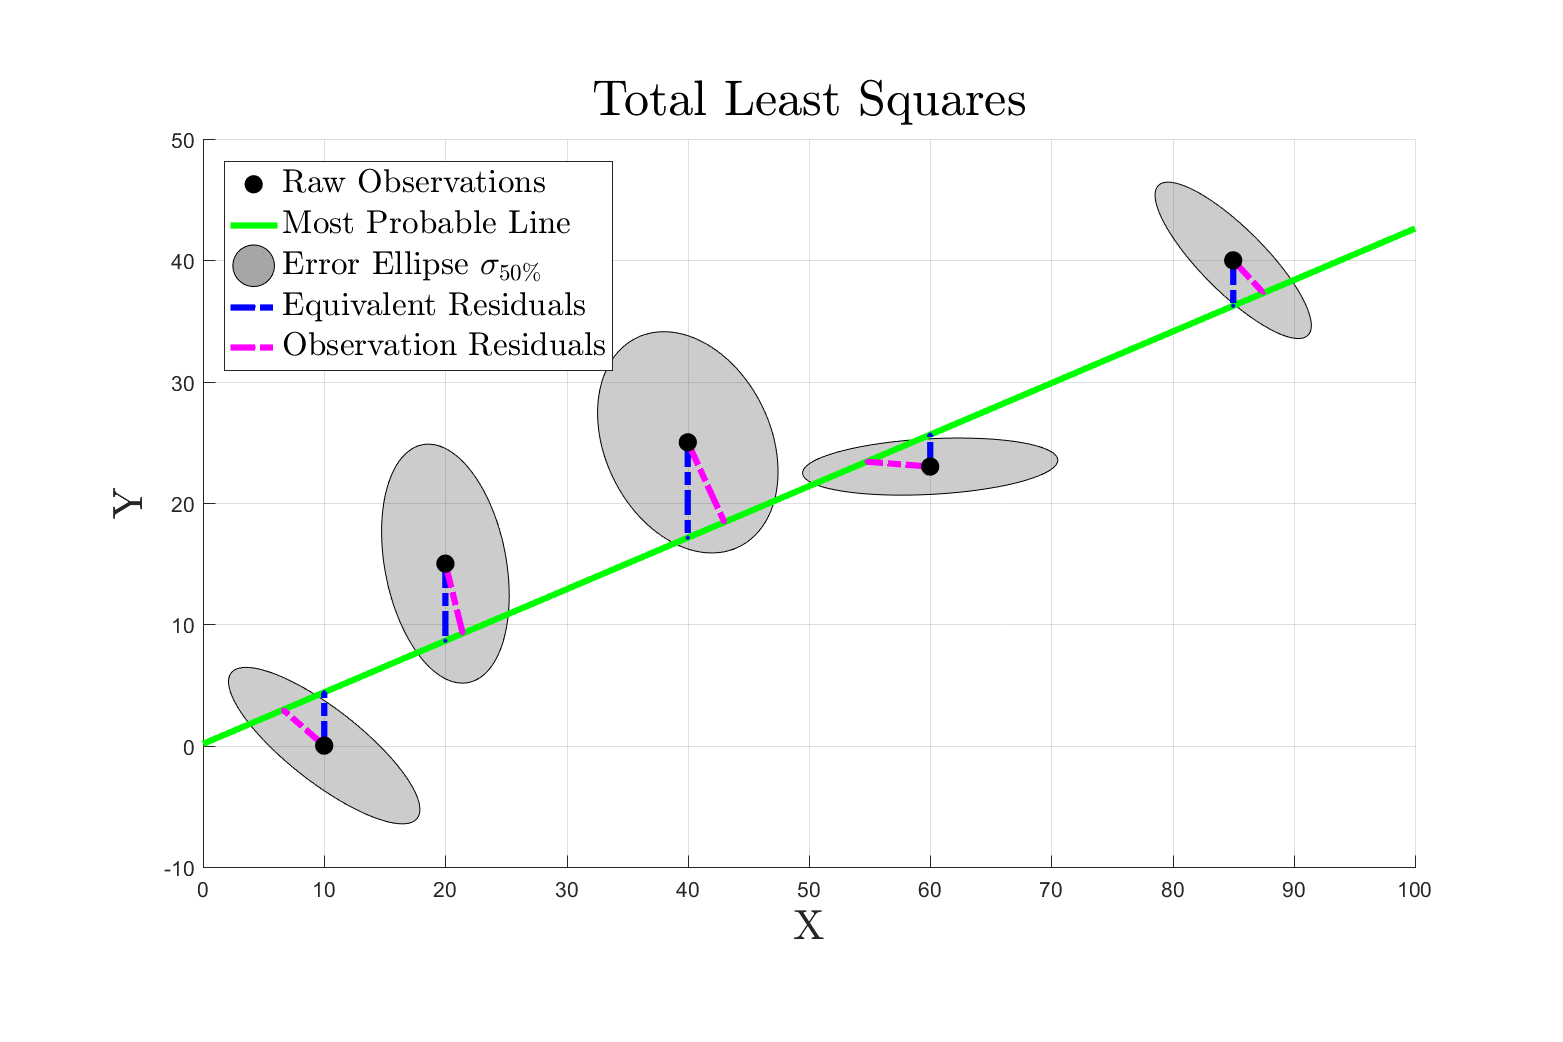
\includegraphics[height = 4in]{TLSexampleA.png}
\end{figure}


Notice how the observation residuals are not just in the y dimension.  OLS is calculated with the same data, and plotted below for comparison.

\begin{figure}[H]
	\centering
	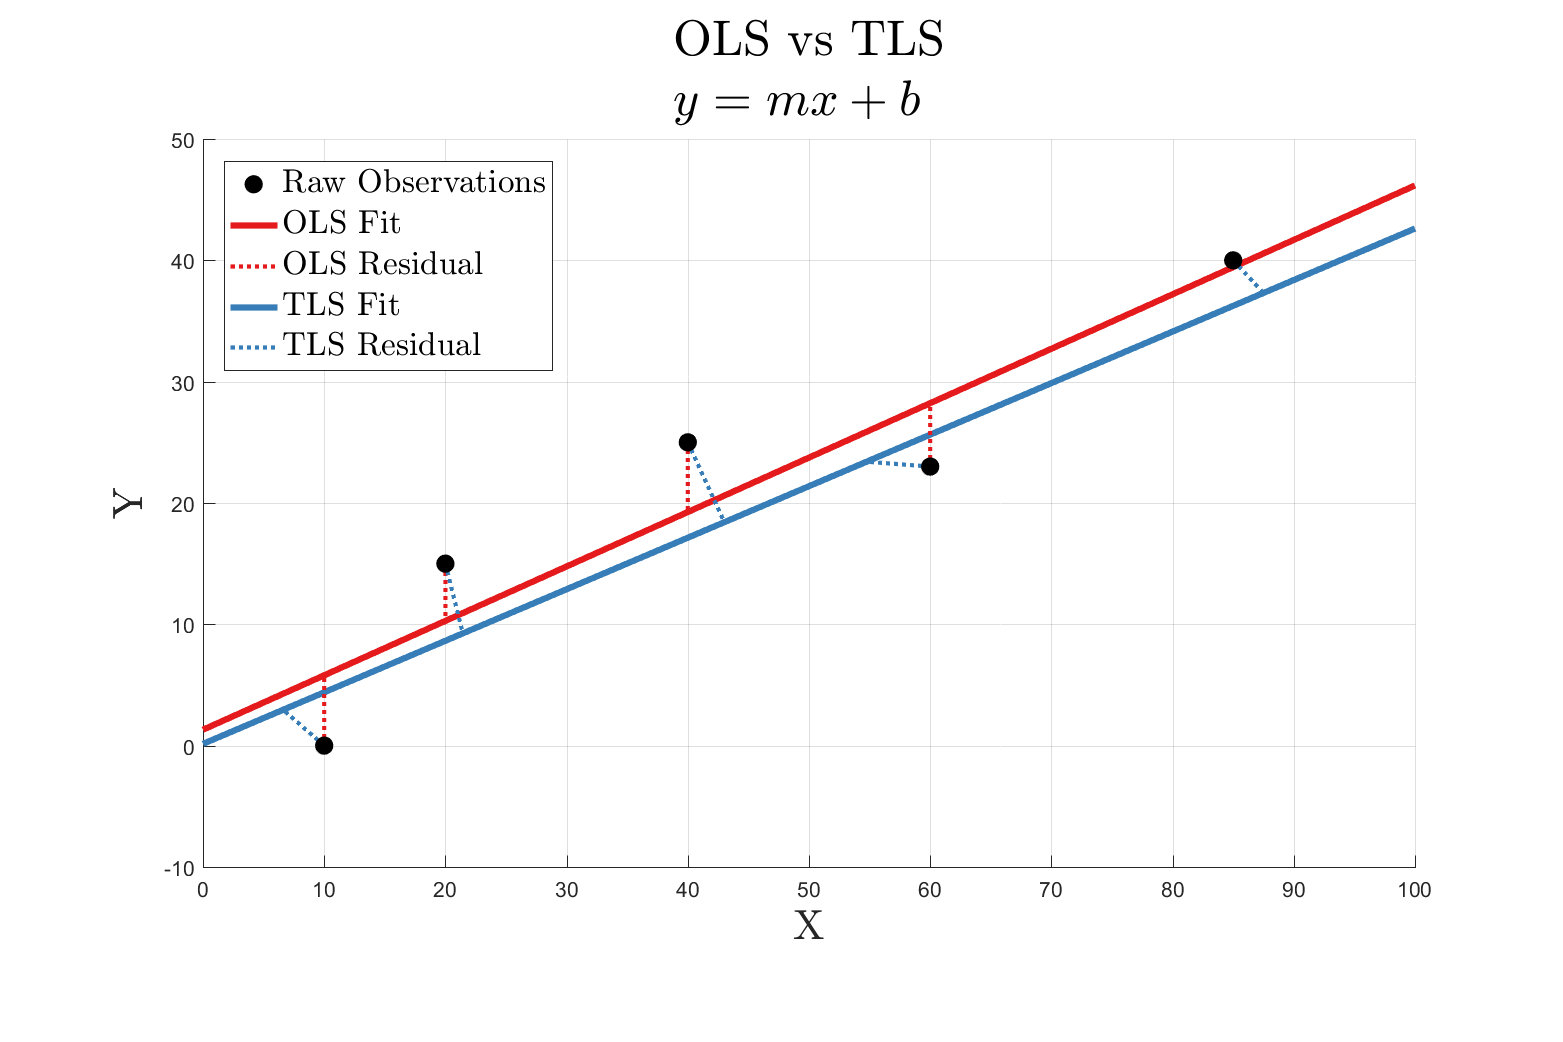
\includegraphics[height = 4in]{TLSexampleB.png}
\end{figure}
\clearpage
\subsection{Example Matlab Code}
\lstinputlisting[
label      = {alg:exampleTLS},
caption    = {exampleTLS.m},
style      = Matlab-editor,
basicstyle = \mlttfamily,
firstline  = 1,
lastline   = 34,
firstnumber= 1
]{exampleTLS.m}

Note: Matlab does not have a built in TLS function, but I wrote a function called LSRTLS.m

\lstinputlisting[
label      = {alg:exampleTLS2},
caption    = {exampleTLS.m: Using lsrtls.m and anonymous function handles to perform TLS.},
style      = Matlab-editor,
basicstyle = \mlttfamily,
firstline  = 36,
lastline   = 40,
firstnumber= 36
]{exampleTLS.m}